\documentclass{article}

\usepackage[utf8]{inputenc}
\usepackage{graphicx}
\usepackage{url}
\usepackage{color}
\usepackage{titlesec}
\usepackage{amsmath}
\usepackage{physics}
\usepackage{amsfonts}
\graphicspath{{../figures/}}

\title{paper draft: supersat}
\author{K. Latimer}
\date{Jan 13, 2020}

\begin{document}

\maketitle


\section{Introduction}
introductory notes.
\section{Theory + Simulation}
\begin{itemize}
	\item brief statement of quasi steady state formula 
	\item we see agreement between actual and QSS supersaturation under the conditions (see figs \ref{wrfvsqssunpoll} and \ref{wrfvsqsspoll}):
	\begin{itemize}
		\item T \textgreater 273K (we're not including ice in the theory)
		\item w \textgreater 2 m/s (reasonably strong updrafts)
		\item cloud LWC \textgreater 1e-4 g/g (in the convection core)
	\end{itemize}
	\item *to discuss* don't see the same distinction as from CAIPEEX between bulk and edge wrt high supersaturation values (see figs \ref{wrfsshistunpoll} and \ref{wrfsshistpoll})
\end{itemize}
\begin{figure}[ht]
    \centering
    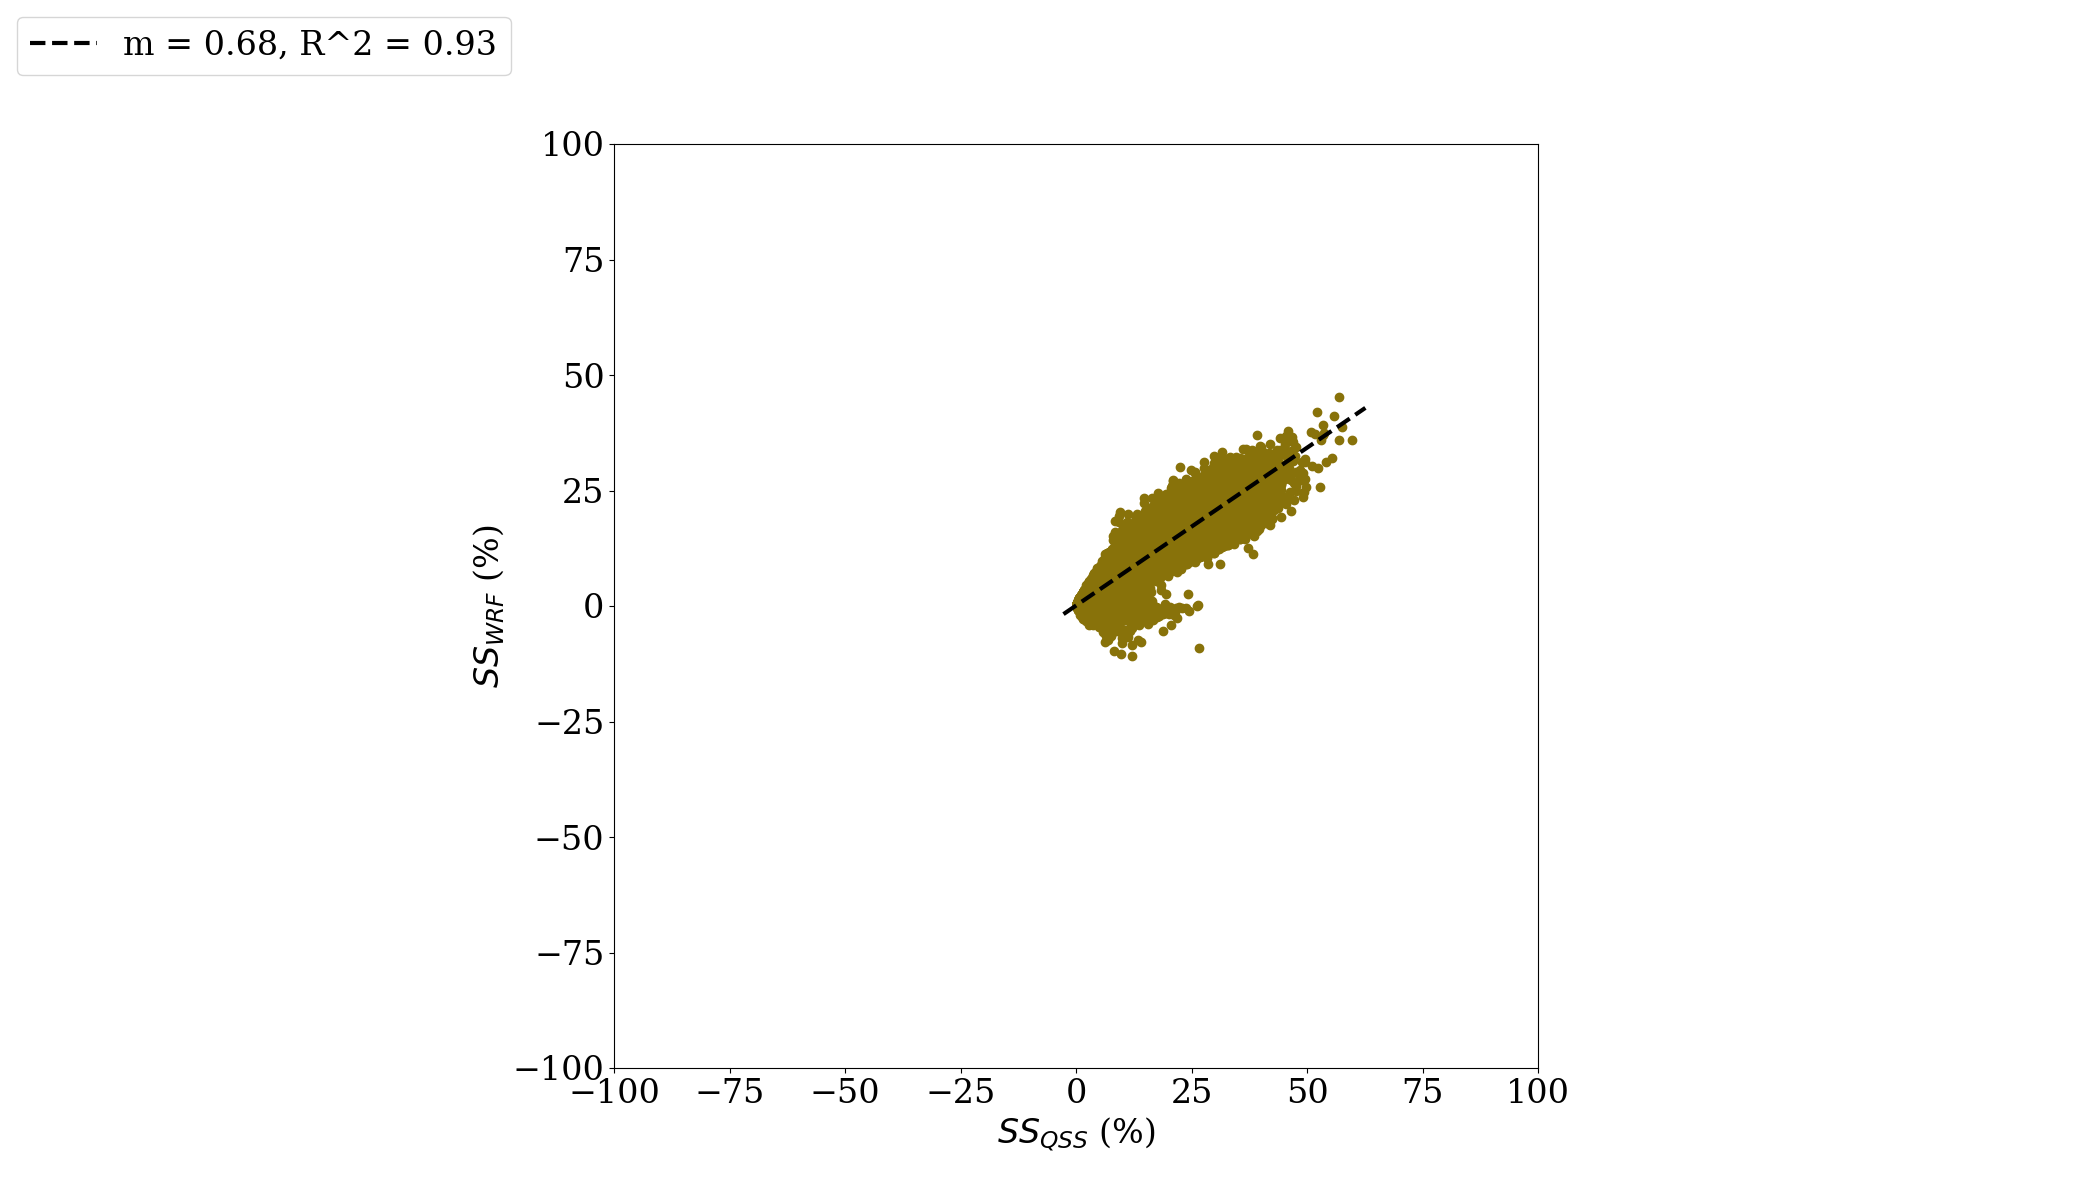
\includegraphics[width=9cm]{mywrf/v28_inclrain_and_vent_qss_vs_fan_Unpolluted_figure.png}
    \caption{Actual ($SS_{WRF}$) vs predicted ($SS_{QSS}$) supersaturation in unpolluted case.}
    \label{wrfvsqssunpoll}
\end{figure}
\begin{figure}[ht]
    \centering
    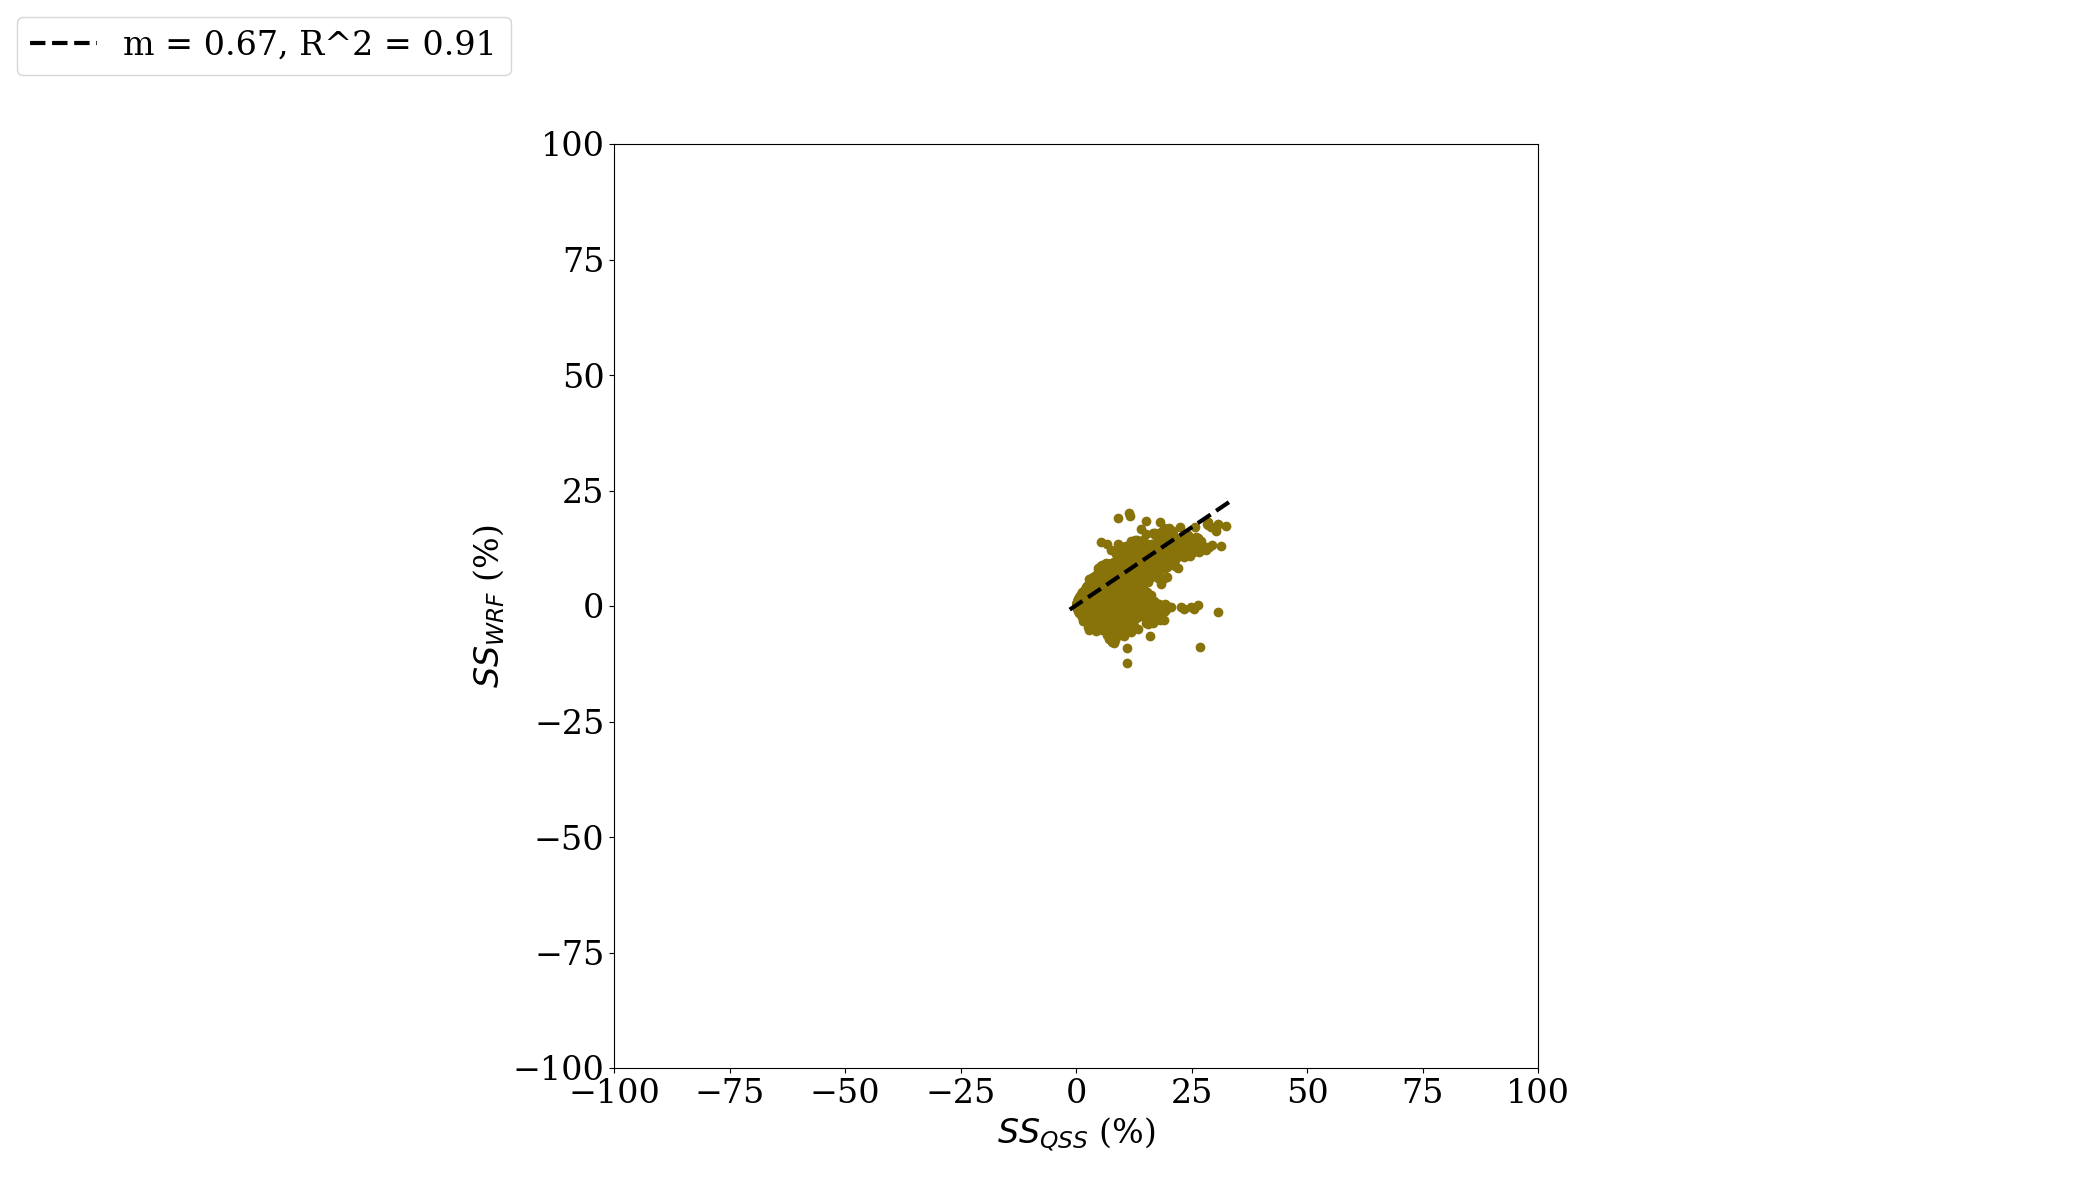
\includegraphics[width=9cm]{mywrf/v28_inclrain_and_vent_qss_vs_fan_Polluted_figure.png}
    \caption{Actual ($SS_{WRF}$) vs predicted ($SS_{QSS}$) supersaturation in polluted case.}
    \label{wrfvsqsspoll}
\end{figure}
\begin{figure}[ht]
    \centering
    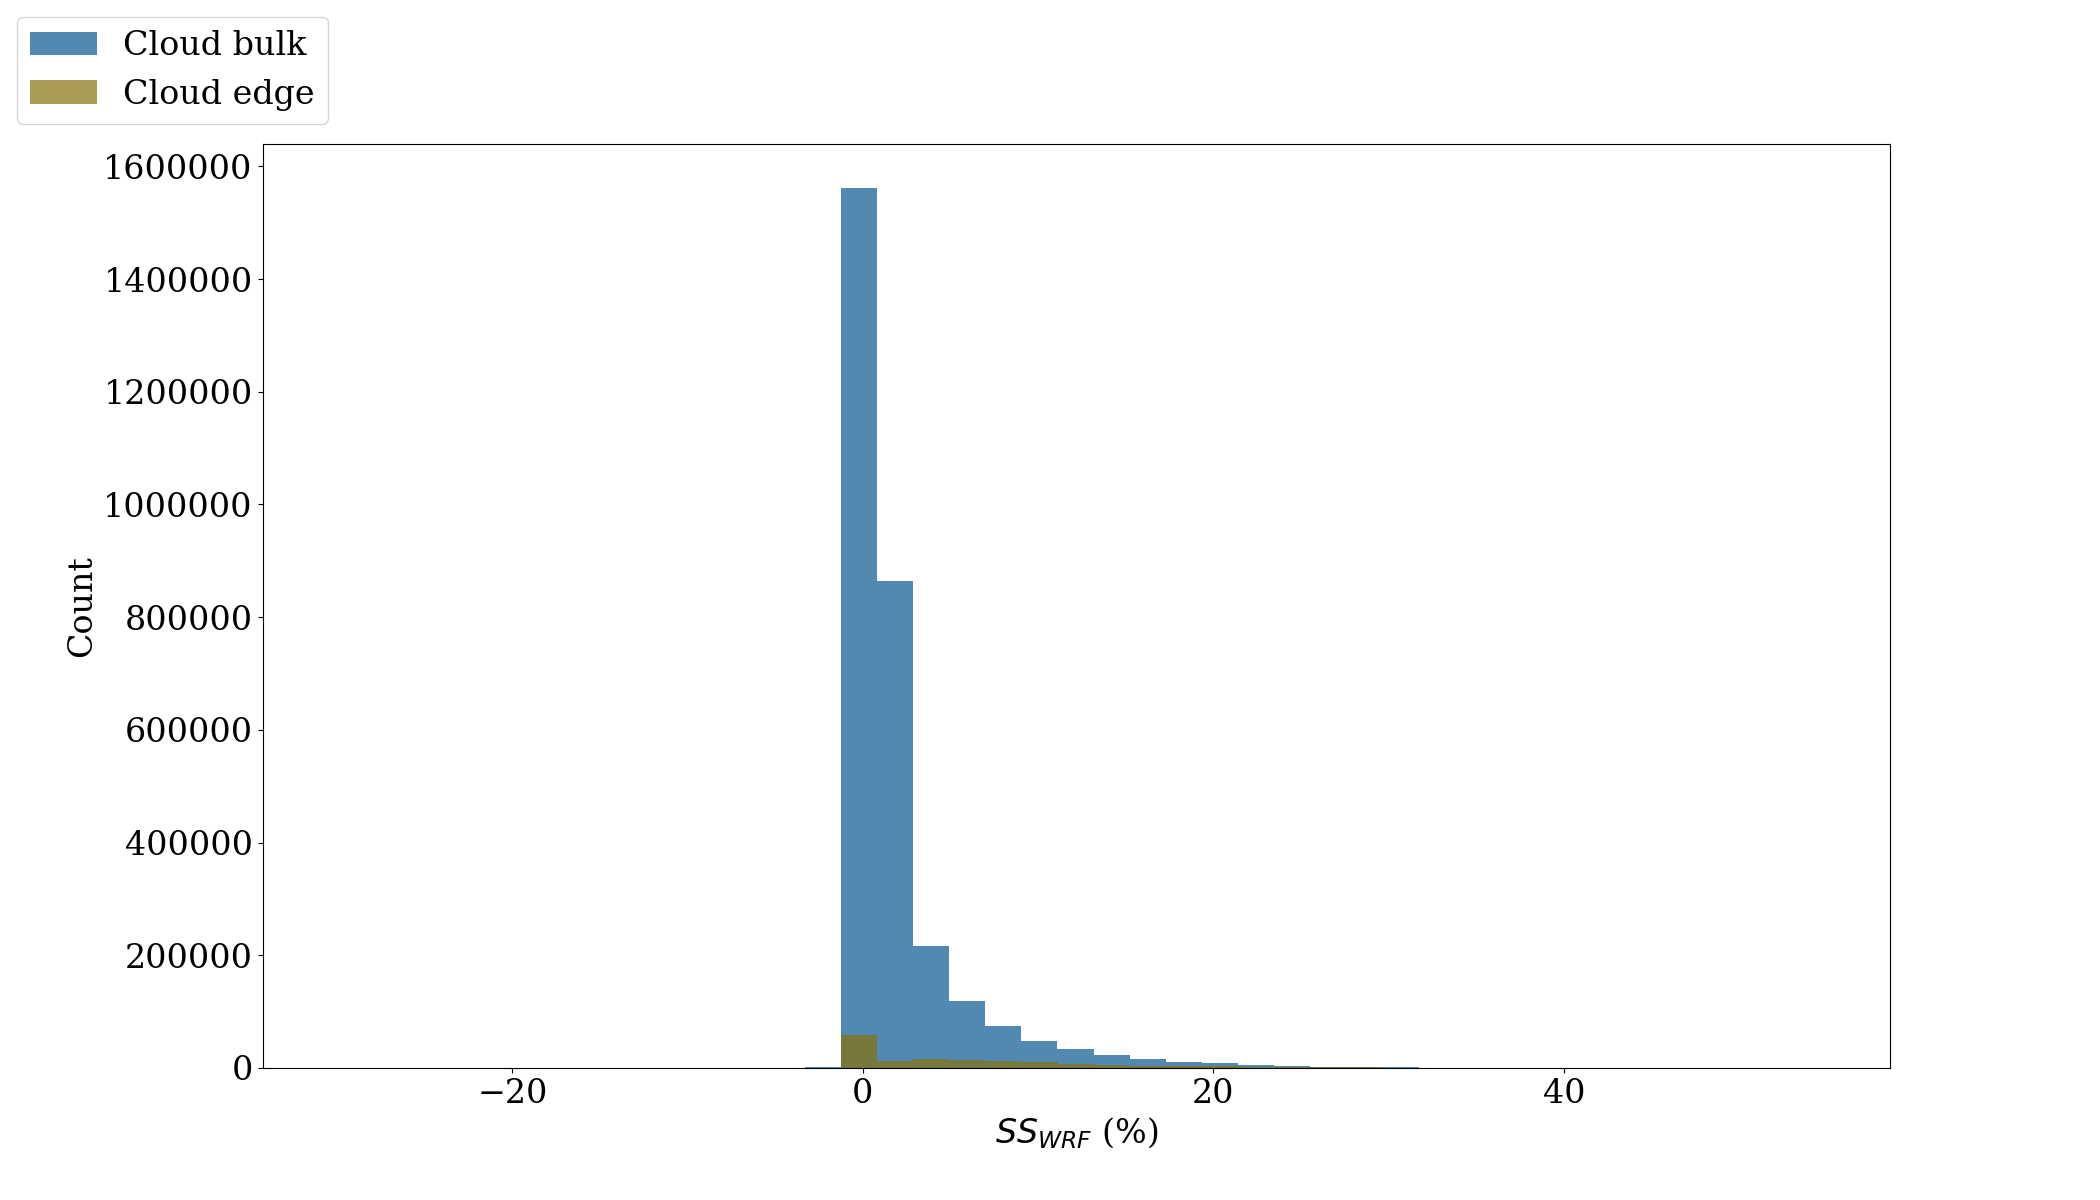
\includegraphics[width=9cm]{mywrf/v13_inclrain_and_vent_bulkedge_hist_Unpolluted_figure.png}
    \caption{Actual ($SS_{WRF}$) supersaturation distribution in unpolluted case. ``Edge" points are lowest 5th percentile LWC of all cloud points in the same altitude slice.}
    \label{wrfsshistunpoll}
\end{figure}
\begin{figure}[ht]
    \centering
    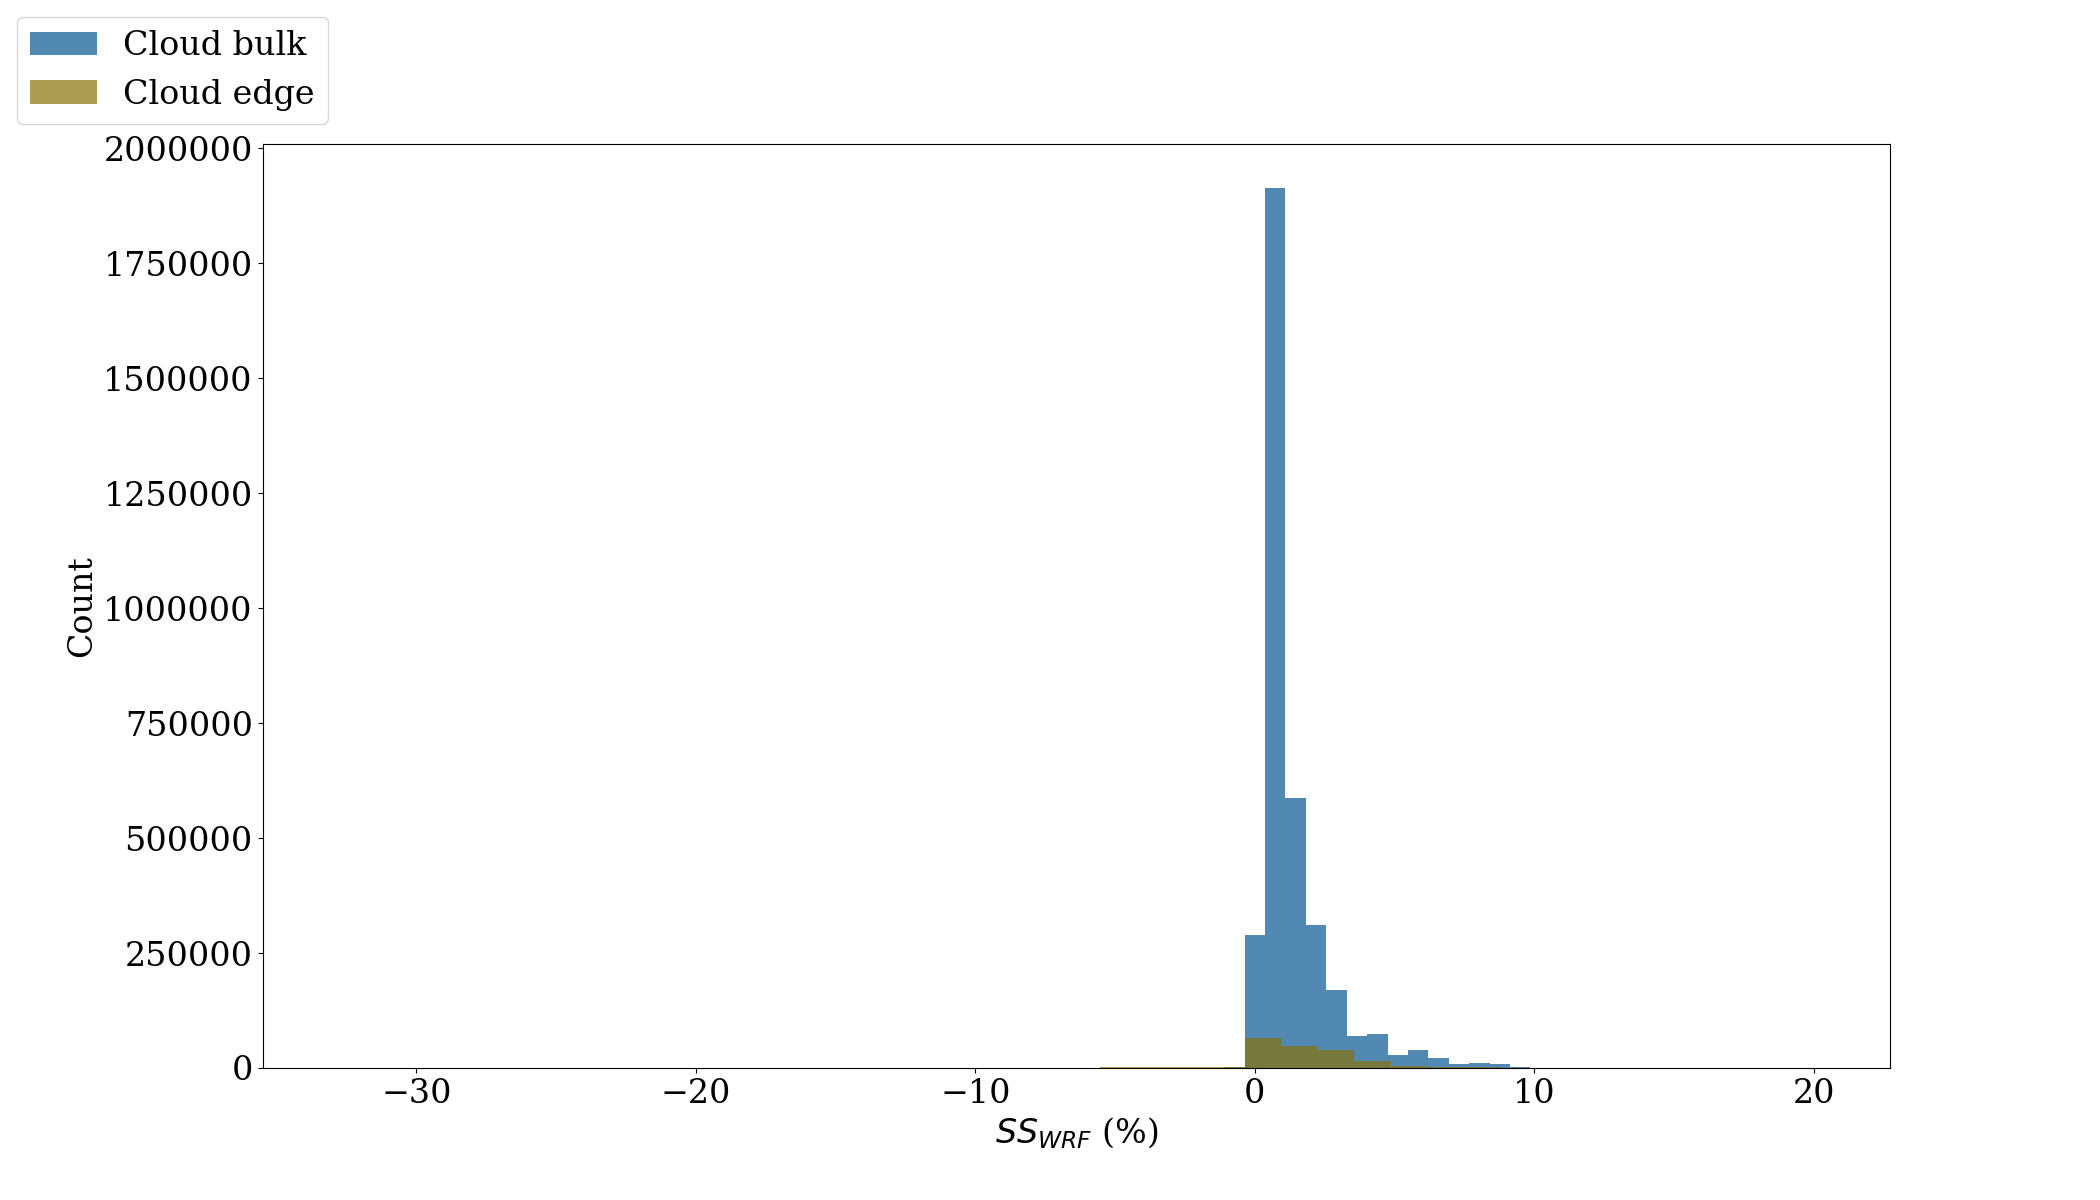
\includegraphics[width=9cm]{mywrf/v13_inclrain_and_vent_bulkedge_hist_Polluted_figure.png}
    \caption{Actual ($SS_{WRF}$) supersaturation distribution in polluted case. ``Edge" points are lowest 5th percentile LWC of all cloud points in the same altitude slice.}
    \label{wrfsshistpoll}
\end{figure}

\section{Experimental data}
\begin{itemize}
	\item using criteria from second bullet point of section 2, $SS_{QSS}$ distribution from HALO data looks like fig \ref{haloqsshist}. 
	\item using criteria from second bullet point of section 2, $SS_{QSS}$ distribution from CAIPEEX data looks like fig \ref{caipeexqsshist}. 
\end{itemize}
\begin{figure}[ht]
    \centering
    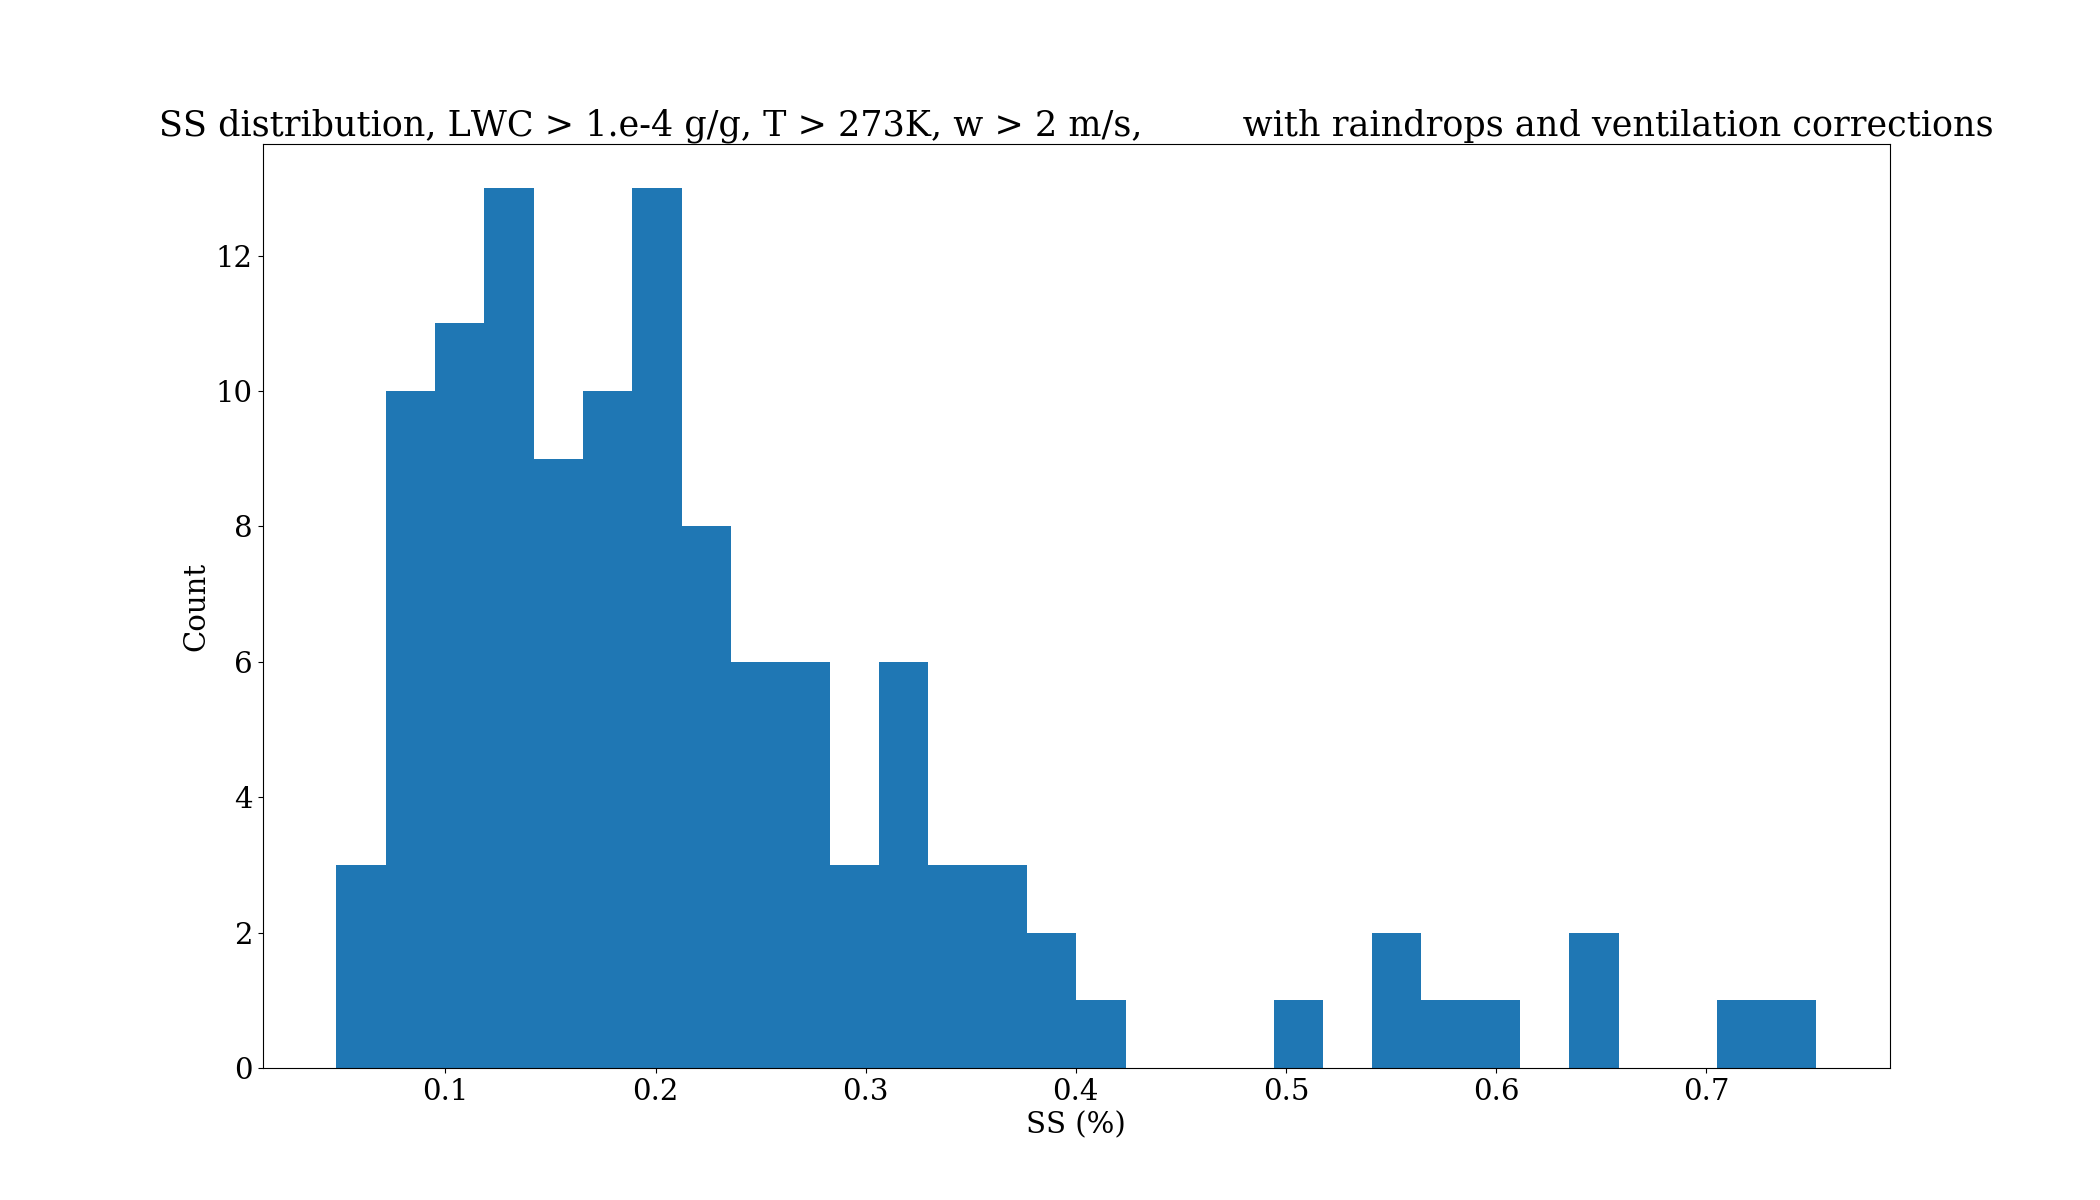
\includegraphics[width=9cm]{halo/v3_ss_with_cip_from_cas_alldates_figure.png}
    \caption{Predicted ($SS_{QSS}$) supersaturation distribution from HALO field campaign (all flight dates). Using filtering criteria outlined in section 2.}
    \label{haloqsshist}
\end{figure}
\begin{figure}[ht]
    \centering
    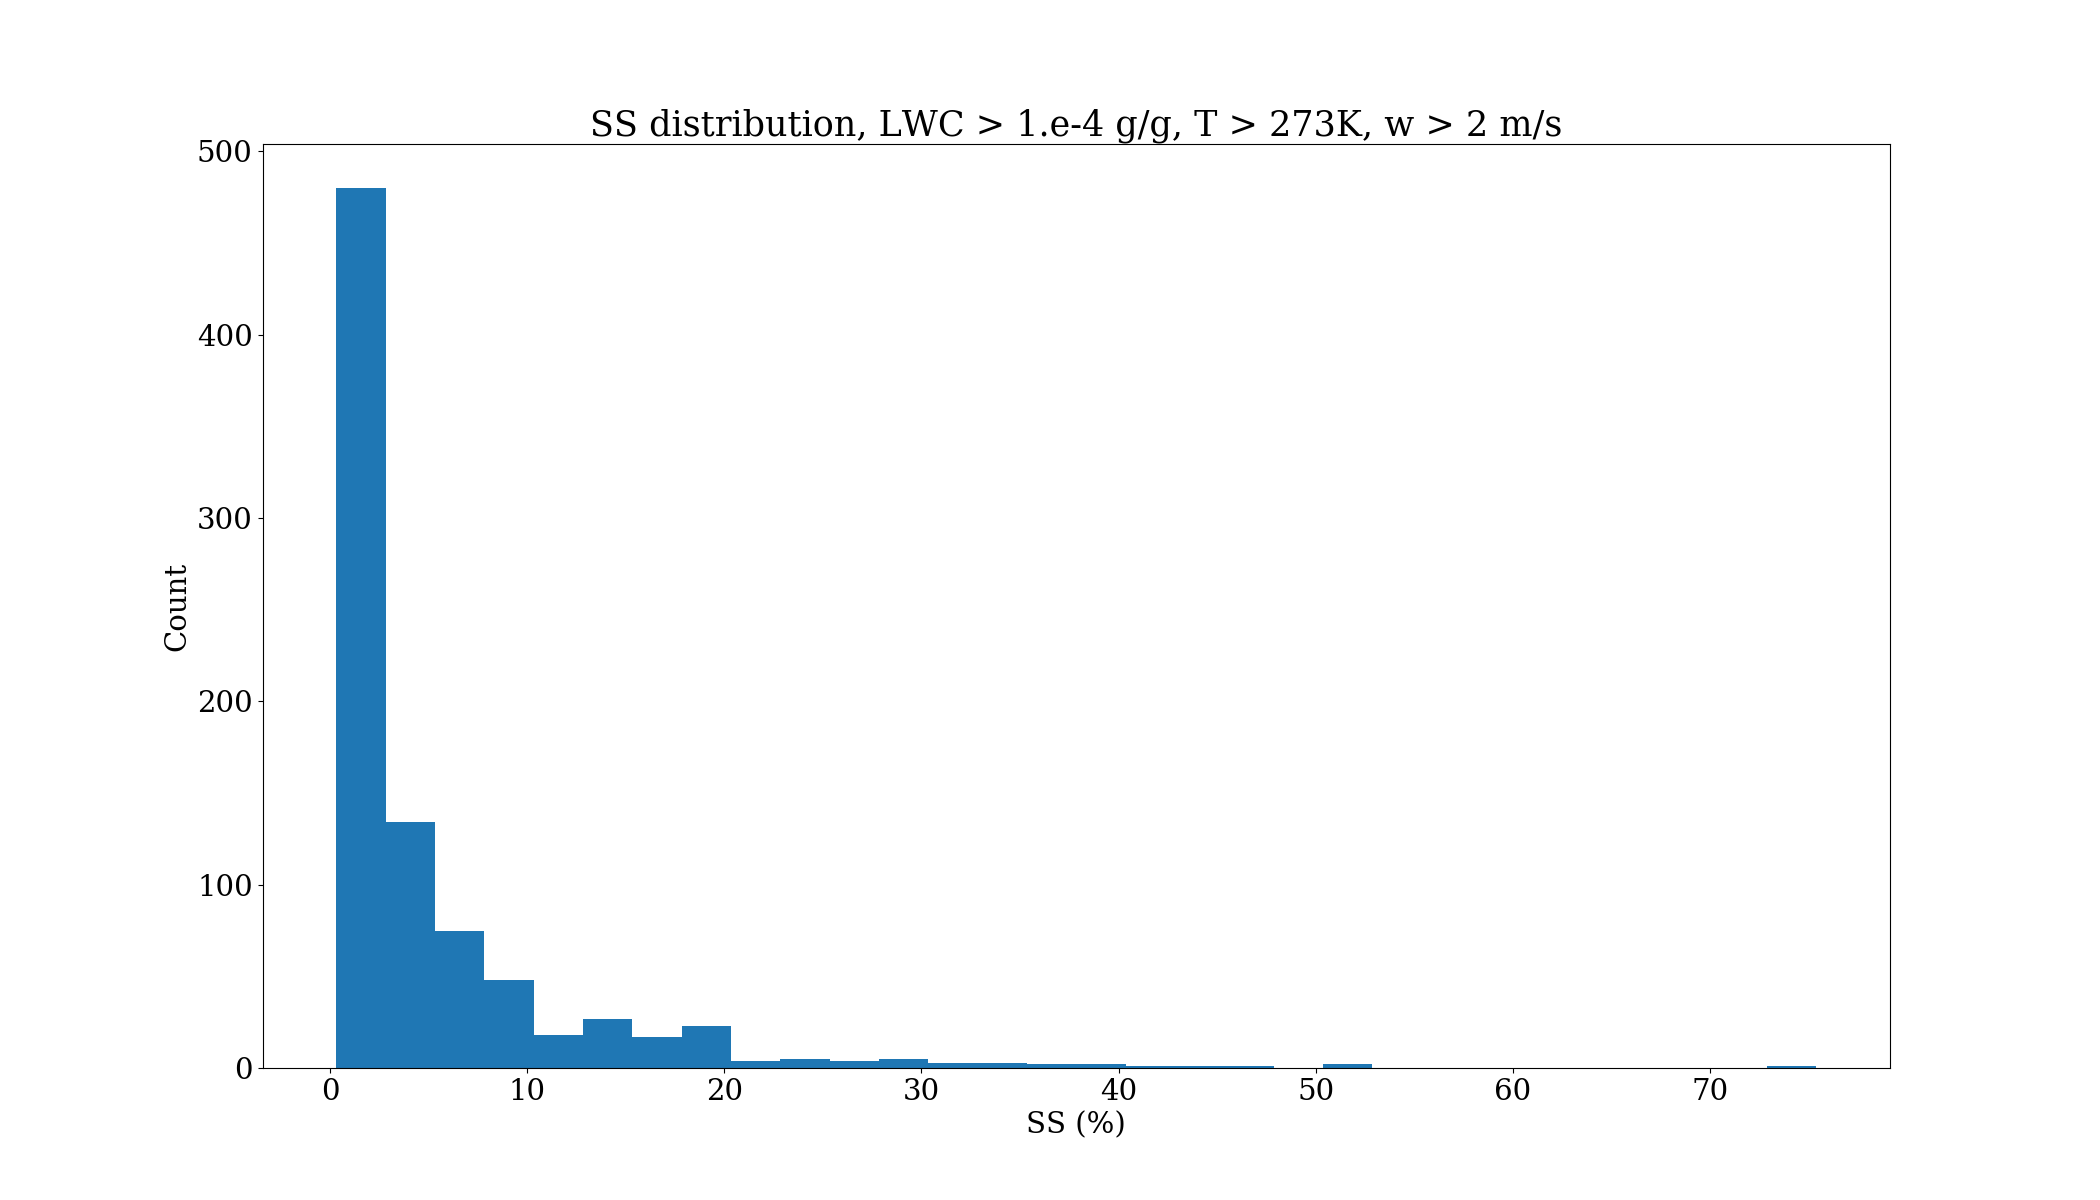
\includegraphics[width=9cm]{caipeex/v1_ss_from_dsd_alldates_figure.png}
    \caption{Predicted ($SS_{QSS}$) supersaturation distribution from CAIPEEX field campaign (all flight dates). Using filtering criteria outlined in section 2, but not including rain drops or ventilation corrections due to lack of data.}
    \label{caipeexqsshist}
\end{figure}
\section{TODO / remaining questions}
\begin{itemize}
	\item equivalent of figs \ref{wrfsshistpoll} / \ref{wrfsshistunpoll} for experimental data
	\item error analysis for experimental data
	\item look into commensurate binning in simulation / experiment comparisons?
	\item analytical justification for why actual and QSS supersaturation is still in linear relation
	\item how much do HALO and CAIPEEX histograms change taking out raindrops / ventilation corrections?
\end{itemize}
This is a reference \cite{Fan2018}.
%\begin{figure}[h]
%    \centering
%    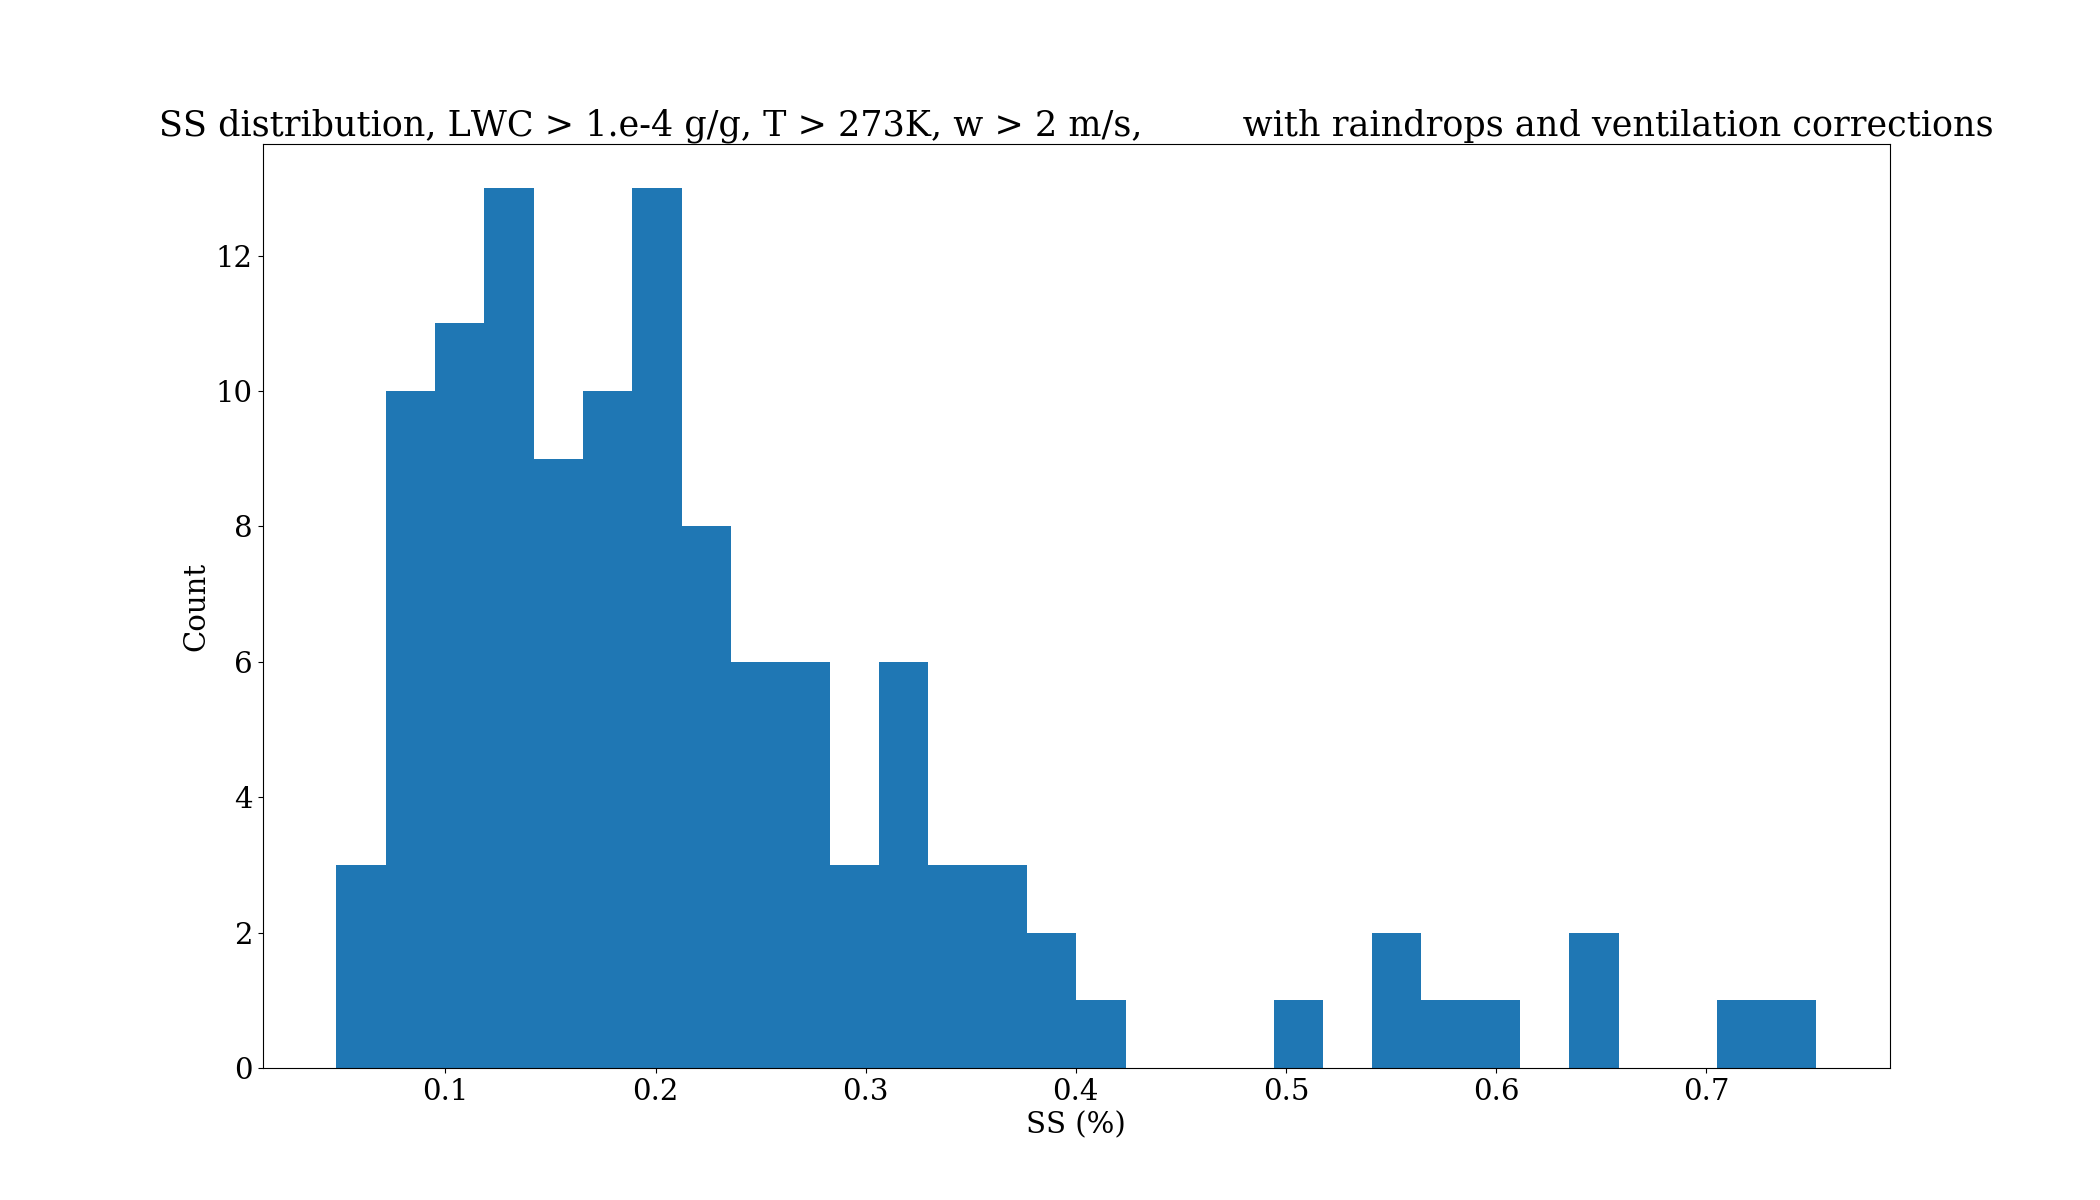
\includegraphics[width=9cm]{halo/v3_ss_with_cip_from_cas_alldates_figure.png}
%    \caption{}
%    \label{fig:fig_label}
%\end{figure}

\bibliography{refs}
\bibliographystyle{ieeetr}
\end{document}
